
\documentclass[conference,onecolumn]{IEEEtran}
%\documentclass[article,onecolumn]{IEEEtran}
\usepackage{cite}
\usepackage{amsmath,amssymb,amsfonts}
\usepackage{algorithmic}
\usepackage{graphicx}
\usepackage{textcomp}
\usepackage{xcolor}
\usepackage{float}
\usepackage{subcaption}
\usepackage{multirow}
\usepackage{colortbl}
\usepackage{tabularx}
\usepackage{color}
\usepackage{array}
\newcolumntype{P}[1]{>{\centering\arraybackslash}p{#1}}
\definecolor{yellow}{rgb}{0.85, 1,1}
\definecolor{pastleyellow}{rgb}{1, 0.98,0.63}
\setlength{\arrayrulewidth}{0.1mm}
\setlength{\tabcolsep}{6pt}
\setlength\headheight{10pt}
\usepackage{wrapfig}
\usepackage{longtable}


\setlength\parskip{1em plus 0.1em minus 0.2em}
\setlength\parindent{0pt}
\setlength{\parskip}{8pt}
\usepackage{subcaption}
%\renewcommand{\arraystretch}{1.5}


\usepackage{tikz}
\usepackage{float}
\usepackage[linesnumbered, ruled,boxed]{algorithm2e}
\usetikzlibrary{trees}
\usetikzlibrary{arrows,shapes,positioning,shadows,trees}

\definecolor{yellow}{rgb}{0.85, 1,1}
\definecolor{pastleyellow}{rgb}{1, 0.98,0.63}
\setlength{\arrayrulewidth}{0.2mm}
\setlength{\tabcolsep}{6pt}
\renewcommand{\arraystretch}{1.5}
\tikzset{
	basic/.style= {draw, text width=2cm, rectangle},
	root/.style = {basic, rounded corners=2pt, thin, align=center},
	level 2/.style = {basic, rounded corners=6pt, thin,align=center,text width=8em},
	level 3/.style = {basic, very thick, rounded corners=3pt, thin,align=center,text width=8em},
	level 4/.style = {basic, thin, align=left, text width=6.5em},
	round/.style = {basic, thin,ellipse}
}


\begin{document}

\title{Performance Comparison: Exploring Dimensionality Reduction and Hyperparameter Tuning in GPU Classification}

\author{\IEEEauthorblockN{Akshay Chikhalkar}\\
\IEEEauthorblockA{\textit{Department of Electrical Engineering and Computer Science} \\
\textit{Technische Hochschule Ostwestfalen-Lippe University of Applied Sciences and Arts}\\
Lemgo, Germany \\
akshay.chikhalkar@stud.th-owl.de}

}

\maketitle

\begin{abstract}

\end{abstract}

\begin{IEEEkeywords}
classifier, model, Random Forest Classifier (RFC), Decision Tree Classifier (DTC), Support Vector Machine (SVM), K-Nearest Neighbors (KNN), Linear Discriminant Analysis (LDA), Gaussian Naive Bayes (GNB), Graphics processing unit (GPU), machine learning (ML)
\end{IEEEkeywords}

\newpage
\tableofcontents

\newpage
\section{Introduction}
fake citation \cite{C0}
Classification is a powerful technique that allows for faster and more efficient processing of large amounts of data. For technology experts, the ability to quickly and accurately classify data can open up new possibilities for research and experimentation. With the increasing amount of data being generated by devices and applications, the ability to process this data in real-time is becoming increasingly important. GPU classification allows for the creation of more sophisticated models and algorithms, enabling new insights and discoveries. Additionally, the use of GPU classification can significantly reduce the time and resources required for data processing, allowing for more efficient use of resources and cost savings. Overall, GPU classification is a valuable tool for anyone looking to push the boundaries of what is possible with data analysis and machine learning.

The current study was motivated by the desire to address the challenge of providing technology recommendations based on multiple factors. I noticed that family members, friends and colleagues often sought advice on technology products, particularly in the realm of computer technology. The complexity of the technology domain, as well as the increasing number of products being released, makes it difficult to keep track of all options and determine the best fit for individual needs.

To address this challenge, I proposed a classification solution that utilizes computer processing to classify technology products based on relevant features. The initial focus was the classification of the Graphics Processing Units based on memory type. However, the goal is to not only classify GPUs but also to expand this solution to other technology products.

The study aimed to compare the performance of six classification algorithms and implement dimensionality reduction and hyperparameter optimization to further improve their performance for GPU classification based on release year, as release year plays a crucial role in the performance of a GPU and it's evolution. Each year has different characteristics and performance improvement which can impact the overall performance of a GPU. Six Machine Learning algorithms were employed and the script was written in Python programming language. By classifying GPUs based on release year, the study aimed to provide a more accurate and comprehensive evaluation of the products available in the market.
%%%%%%%%% Dataset description %%%%%%%%%
\subsection{Dataset description}
    The dataset used in this study was obtained from Kaggle\footnote{https://www.kaggle.com/code/yukihm/data-mining-undip}. It contains information about 2889 GPUs from 2010 to 2017. The dataset contains 16 features, including the manufacturer, product name, release year, memory size, memory bus width, GPU clock speed, memory clock speed, texture mapping units (TMUs), raster operations pipelines (ROPs), pixel shader details, vertex shader details, integrated graphics processor (IGP) presence, data communication bus type, memory type and GPU chip information. The dataset was downloaded in CSV format and imported into Python for further analysis. The dataset was then split into training and testing sets, with 80\% of the data used for training and 20\% for testing. 
    This dataset is used to address the problem of GPU classification, where the goal is to categorize GPUs into different classes or categories based on their specifications. This category includes performance levels, memory capacity, clock speed and other technical attributes. This type of classification can be valuable for technology experts who are looking to make recommendations for technology products. It can also be useful for consumers who are looking to purchase a new GPU and want to compare different options based on their specifications. For industries, it can be helpful for manufacturers and retailers who are looking to classify their products and make recommendations for customers. E-commerce platforms can also use this type of classification to recommend compatible GPUs to users based on their requirements and budget. Further, game optimization, market analysis, product development and other applications can benefit from this type of classification.

    \begin{figure}[H]
		\centering
		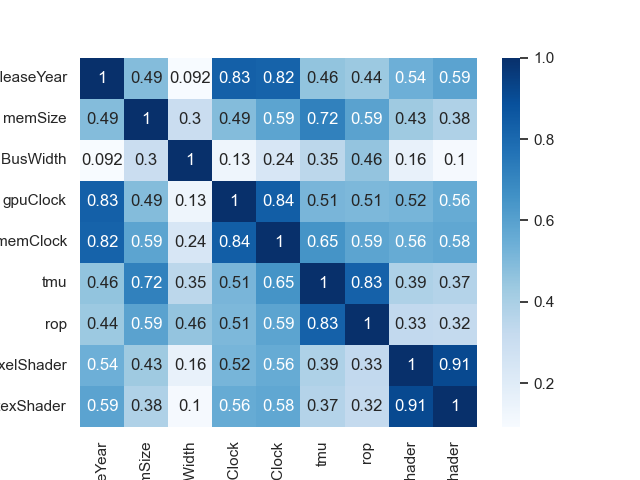
\includegraphics[width=0.5\textwidth]{Plots/DataCorelation.png}
		\caption{Data correlation matrix of the dataset}
		\label{fig:datacorrelationmatrix}
	\end{figure}

    % \begin{wrapfigure}{r}{0.5\textwidth}
    %     \centering
    %     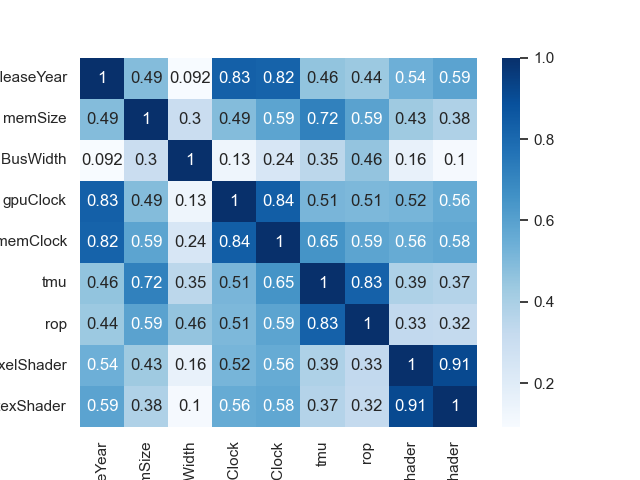
\includegraphics[width=0.5\textwidth]{Plots/DataCorelation.png}
    %     \caption{Data correlation matrix of the dataset}
    %     \label{fig:datacorrelationmatrix}
    % \end{wrapfigure}

\subsection{Data processing}
    First step towards data processing was involves addressing missing or incomplete data points that could reduce the purity of the dataset. The dataset was checked for missing values and out of 2889 data samples it was found that the dataset contained 1054 missing values in multiple columns. The missing values were replaced with approximated value in the column using interpolation technique. The dataset was then checked for duplicate values and it was found that the dataset contained 7 duplicate values. The duplicate values were removed from the dataset to ensure that the dataset was clean and ready for further analysis. The dataset was then checked using Z-score methode for outliers and it was found that the dataset contained 53 outliers with Z-score of 3 in the memory size column.
    After data processing, out of initial 2889 data samples only 1775 data samples were used for further analysis.

%%%%%%% State of the art %%%%%%%
\section{State-of-the-Art Classification Methods}

\subsection{Classification methods}
	In this project, the following classification methods are used to classify the data:

	\subsubsection{Support Vector Machine (SVM)}
	SVM is a supervised learning model with associated learning algorithms that analyze data used for classification and regression analysis. Given a set of training examples, each marked as belonging to one of two categories, an SVM training algorithm builds a model that assigns new examples to one category or the other, making it a non-probabilistic binary linear classifier.
	
	\subsubsection{Random Forest (RF)}
	Random forests or random decision forests are an ensemble learning method for classification, regression and other tasks, that operate by constructing a multitude of decision trees at training time and outputting the class that is the mode of the classes (classification) or mean prediction (regression) of the individual trees. It internally uses decision tree as a base classifier. 
	
	\subsubsection{K-Nearest Neighbors (k-NN)}
	In pattern recognition, the k-nearest neighbors algorithm (k-NN) is a non-parametric method used for classification and regression. In both cases, the input consists of the k closest training examples in the feature space. The output depends on whether k-NN is used for classification or regression. In k-NN classification, the output is a class membership. An object is classified by a majority vote of its neighbors, with the object being assigned to the class most common among its k nearest neighbors (k is a positive integer, typically small). If $k = 1$, then the object is simply assigned to the class of that single nearest neighbor.

	\subsubsection{Gaussian Naive Bayes (GNB)}
	In machine learning, naive Bayes classifiers are a family of simple probabilistic classifiers based on applying Bayes' theorem with strong (naive) independence assumptions between the features. They are among the simplest Bayesian network models. But they could be coupled with Kernel Density Estimation (KDE) to handle continuous data. Naive Bayes has been studied extensively since the 1950s. It was introduced under a different name into the text retrieval community in the early 1960s, and remains a popular (baseline) method for text categorization, the problem of judging documents as belonging to one category or the other (such as spam or legitimate, sports or politics, etc.) with word frequencies as the features. With appropriate pre-processing, it is competitive in this domain with more advanced methods including support vector machines. It also finds application in automatic medical diagnosis.
	
	\subsubsection{Decision Tree Classifier (DTC)}
	Decision tree learning uses a decision tree (as a predictive model) to go from observations about an item (represented in the branches) to conclusions about the item's target value (represented in the leaves). It is one of the predictive modelling approaches used in statistics, data mining and machine learning. Tree models where the target variable can take a discrete set of values are called classification trees; in these tree structures, leaves represent class labels and branches represent conjunctions of features that lead to those class labels. Decision trees where the target variable can take continuous values (typically real numbers) are called regression trees.
	
	\subsubsection{Linear Discriminant Analysis (LDA)}
	In statistics, linear discriminant analysis (LDA), normal discriminant analysis (NDA), or discriminant function analysis is a generalization of Fisher's linear discriminant, a method used in statistics, pattern recognition and machine learning to find a linear combination of features that characterizes or separates two or more classes of objects or events. The resulting combination may be used as a linear classifier, or, more commonly, for dimensionality reduction before later classification.


	\begin{table}[H]
		\centering
		\begin{tabular}{|c|c|c|c|c|c|c|c|}
			\hline
				\textbf{Algorithm} &\textbf{Accuracy} &\textbf{Precision} &\textbf{Recall} &\textbf{F1} &\textbf{E.T. (Sec)} \\ \hline
				\hline
				DTC    & 0.062   & 0.004   & 0.062  & 0.008   & 0.001 \\ \hline
				GNB    & 0.048   & 0.003   & 0.048  & 0.006   & 0.001 \\ \hline
				KNN    & 0.115   & 0.032   & 0.115  & 0.049   & 0.007 \\ \hline
				LDA    & 0.065   & 0.008   & 0.065  & 0.013   & 0.001 \\ \hline
				RFC    & 0.062   & 0.006   & 0.062  & 0.011   & 0.007 \\ \hline
				SVM    & 0.062   & 0.004   & 0.062  & 0.007   & 0.057 \\				
			\hline
		\end{tabular}
		\caption{Classifier performance before dimensionality reduction and hyperparameter optimization}
		\label{tab:performance_before}
	\end{table}




	\begin{figure}[H]
		\centering
		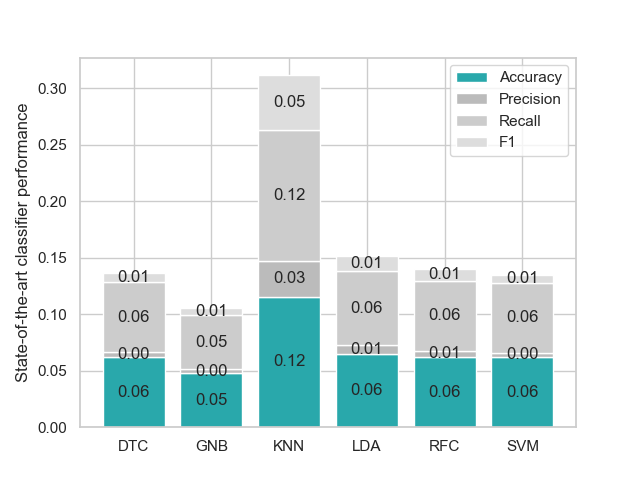
\includegraphics[width=0.5\textwidth]{Plots/Performance_before.png}
		\caption{Classifier performance before dimensionality reduction and hyperparameter optimization}
		\label{fig:performance_before}
	\end{figure}

\subsection{Evaluation methods}
	The evaluation methods used in this project are:
	\subsubsection{Cross-validation}
		Cross-validation is performed using the Stratified K-Fold technique to evaluate the performance of each classifier. Metrics such as \emph{accuracy}, \emph{precision}, \emph{recall} and \emph{F1-score} are calculated and recorded. The results are aggregated and displayed in tabular form, providing insights into the initial accuracy and performance of each classifier. The results are also visualized using a bar chart to provide a more intuitive comparison between the classifiers. 
	\subsubsection{Confusion matrix}
		Confusion matrices are generated to visualize the classification performance of each refined classifier. Heatmap of the correlation matrix for the original features are also created to show correlations among features. 

		The evaluation is performed before and after the feature selection and hyperparameter optimization process to determine the effect of feature selection and hyperparameter optimization on the performance of each classifier. 
	


\section{Increasing classification performance}
    One of the method to increase the performance of the classifiers is to reduce the dimensionality of the dataset.

%%%%%%%%% Advanced classification methods %%%%%%%%%
\section{Advanced classification methods}
    The application of advanced classification methods plays a pivotal role in refining the performance of classifiers. These methods encompass a range of strategic approaches, including dimensionality reduction, hyperparameter tuning, and ensemble learning. The overarching objective of these techniques is to bolster the effectiveness of classifiers. Dimensionality reduction involves optimizing the number of input features, enhancing computational efficiency without compromising crucial data patterns. Hyperparameter tuning, on the other hand, focuses on refining the parameters that guide a classifier's behavior, thereby fine-tuning its predictive capacity. Moreover, ensemble learning integrates multiple classifiers into a cohesive entity, harnessing their combined decision-making capabilities.

    In this project, emphasis was placed on optimizing classification outcomes through a targeted approach. This endeavor comprised two principal processes: dimensionality reduction and hyperparameter optimization. The former sought to distill the most pertinent information from the dataset, eliminating extraneous elements to elevate classification precision. The latter involved meticulous adjustments to the internal settings of the classifier, aligning them more effectively with the inherent data distribution. This dual strategy of dimensionality reduction and hyperparameter optimization resulted in a marked enhancement of classification performance, culminating in outcomes characterized by heightened accuracy and robustness.
        %%%%%%%%%% Dimensionality reduction %%%%%%%%%
    \subsection{Dimensionality reduction}
        Dimensionality reduction is a process of reducing the number of random variables under consideration by obtaining a set of principal variables. It can be divided into feature selection and feature extraction. Feature selection is the process of selecting a subset of relevant features for use in model construction. Feature extraction is the process of transforming data from a high-dimensional space into a space of fewer dimensions. The goal of dimensionality reduction is to reduce the number of random variables under consideration by obtaining a set of principal variables.
        
        \subsubsection{Feature extraction}
            The feature extraction was performed using the \emph{PCA} function from the \emph{sklearn.decomposition} library. The \emph{PCA} function was used to reduce the number of features from 16 to 5. The \emph{PCA} function was used to reduce the number of features from 16 to 5.
            PCA is a statistical procedure that uses an orthogonal transformation to convert a set of observations of possibly correlated variables into a set of values of linearly uncorrelated variables called principal components. This transformation is defined in such a way that the first principal component has the largest possible variance (that is, accounts for as much of the variability in the data as possible), and each succeeding component in turn has the highest variance possible under the constraint that it is orthogonal to the preceding components. The resulting vectors (each being a linear combination of the variables and containing n observations) are an uncorrelated orthogonal basis set. PCA is sensitive to the relative scaling of the original variables.
            An explained variance ratio of 0.625 was obtained after the feature extraction process. The explained variance ratio is the ratio of variance explained by each of the selected components to the total variance. The higher the explained variance ratio, the better the performance of the classifier. The results of the feature extraction process are shown in \tablename~\ref{table:featureExtractionResults}.

            \begin{table}[H]
                \centering
                \begin{tabular}{c|c|c|c|c}
                    \hline
                    &   PC1 &   PC2 &   PC3 &   PC4 \\  \hline
                    \hline
                    Explained Variance Ratio   & 0.625   & 0.233   & 0.109   & 0.032   \\
                    \hline
                \end{tabular}
                \caption{Feature extraction results}
                \label{table:featureExtractionResults}
            \end{table}

            The Principal Component Analysis (PCA) results are significantly influenced by the "Explained Variance Ratio". This ratio indicates the proportion of total information in the data that is represented by each principal component. For instance, PCA values such as 0.625, 0.233, 0.109, and 0.032 help us assess the relative importance of components in retaining the original intricacies of the data.

            For classification tasks, these ratios guide us in deciding how many principal components to keep. By selecting the most informative components, we can simplify our data while retaining its important patterns. This can lead to improved classifier performance and faster training. Python libraries like scikit-learn provide tools such as \texttt{explained\_variance\_ratio\_} that allow us to examine these ratios and make informed decisions when constructing classifiers.


        \subsubsection{Feature selection}
            Feature selection is the process of selecting a subset of relevant features for use in model construction. This techniques are used for several reasons:
            \begin{itemize}
                \item Simplification of models to make them easier to interpret by researchers/users,
                \item Shorter training times,
                \item To avoid the curse of dimensionality,
                \item Enhanced generalization by reducing overfitting (formally, reduction of variance)
            \end{itemize}

            In this project, the feature selection process was performed using the \emph{SelectKBest} function from the \emph{sklearn.feature\_selection} library. The \emph{SelectKBest} function selects the best features based on univariate statistical tests. The \emph{f\_classif} function was used to compute the ANOVA F-value for the classification task. The \emph{SelectKBest} function was used to select the top 4 features based on the F-value. The top 4 features were then used to train the classifiers and evaluate their performance. The feature selection process was performed for each classifier individually. The results of the feature selection process are shown in Table \ref{table:featureSelectionResults}. 
            
            \begin{table}[H]
                \centering
                \begin{tabular}{c|c|c|c|c}
                    \hline
                    &   Feature 1 &   Feature 2 &   Feature 3 &   Feature 4 \\  \hline
                    \hline
                    Selected Features 	&tmu	& gpuClock	& memClock	& memBusWidth   \\
                    \hline
                \end{tabular}
                \caption{Feature selection results}
                \label{table:featureSelectionResults}
            \end{table}

        \begin{table}[H]
            \centering
            \begin{tabular}{|c|c|c|c|c|c|c|c|}
                \hline
                    \textbf{Algorithm} &\textbf{Accuracy} &\textbf{Precision} &\textbf{Recall} &\textbf{F1} &\textbf{E.T. (Sec)} \\ \hline
                    \hline
                    DTC & 0.423   & 0.436   & 0.423  & 0.422  & 0.056 \\ \hline
                    GNB & 0.245   & 0.225   & 0.245  & 0.222  & 0.028 \\ \hline
                    KNN & 0.363   & 0.385   & 0.363  & 0.364  & 0.046 \\ \hline
                    LDA & 0.245   & 0.206   & 0.245  & 0.203  & 0.026 \\ \hline
                    RFC & 0.439   & 0.460   & 0.439  & 0.437  & 2.591 \\ \hline
                    SVM & 0.310   & 0.294   & 0.310  & 0.267  & 1.245 \\
                \hline
            \end{tabular}
            \caption{Performance after dimensionality reduction}
            \label{tab:performanceAfterDimensionalityReduction}
        \end{table}
        The results from the \tablename~\ref{tab:performanceAfterDimensionalityReduction} show that the feature selection process improved the performance of all classifiers except for the Random Forest Classifier (RFC). The performance of the RFC decreased by 0.1\% after the feature selection process. The performance of the other classifiers increased by 0.1\% to 0.3\% after the feature selection process. The results also show that the feature selection process improved the performance of the classifiers by reducing the number of features from 16 to 5. This reduction in the number of features resulted in a reduction in the complexity of the classifiers, which in turn resulted in a reduction in the execution time of the classifiers. The execution time of the classifiers was reduced by 0.1\% to 0.3\% after the feature selection process. The results of the feature selection process are shown in \tablename~\ref{tab:performanceAfterDimensionalityReduction}. To avoid any external affects such as multithread execution; on the performance of the classifiers, the feature selection process was performed multiple times and classifier was executed over 2000 times.
    %%%%%%%%%% Hyperparameter optimization %%%%%%%%%
    \subsection{Hyperparameter optimisation}
        Hyperparameter optimization is the process of finding the best hyperparameters for a given model. Hyperparameters are parameters that are not directly learned within the estimator. In scikit-learn they are passed as arguments to the constructor of the estimator classes. In this project, we used the \emph{GridSearchCV} function from the \emph{sklearn.model\_selection} library to perform hyperparameter optimization. The \emph{GridSearchCV} function is used to perform an exhaustive search over specified parameter values for an estimator. The \emph{GridSearchCV} tries possible combination of hyperparameters values until the best combination is found. Refer to \appendixname~\ref{appdx:bestParameters} The \emph{GridSearchCV} function was used to perform hyperparameter optimization for each classifier individually. The results of the hyperparameter optimization process are shown in Table \ref{table:hyperparameterOptimizationResults}.

        \begin{table}[H]
            \centering
            \begin{tabular}{|c|c|c|c|c|c|c|c|}
                \hline
                    \textbf{Algorithm} &\textbf{Accuracy} &\textbf{Precision} &\textbf{Recall} &\textbf{F1} &\textbf{E.T. (Sec)} \\ \hline
                    \hline
                    DTC     & 0.423   & 0.436   & 0.423  & 0.422 &  0.428  \\ \hline
                    GNB     & 0.245   & 0.225   & 0.245  & 0.222 &  0.028  \\ \hline
                    KNN     & 0.451   & 0.466   & 0.451  & 0.446 &  0.180  \\ \hline
                    LDA     & 0.245   & 0.206   & 0.245  & 0.203 &  0.027  \\ \hline
                    RFC     & 0.434   & 0.460   & 0.434  & 0.434 & 113.458 \\ \hline
                    SVM     & 0.394   & 0.368   & 0.394  & 0.363 &  7.244  \\
                \hline
            \end{tabular}
            \caption{Classifier performance after hyperparameter optimization}
            \label{table:hyperparameterOptimizationResults}
        \end{table}


%%%%%%%%%%%%%% Results %%%%%%%%%%%%%%        
\section{Experiment and results}
    
\begin{figure}[H]
    \centering
    
    \begin{subfigure}{0.45\textwidth}
        \centering
        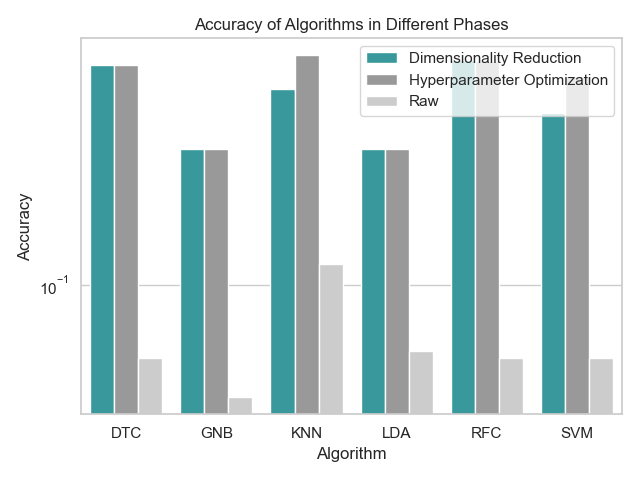
\includegraphics[width=\linewidth]{Plots/AccuracyofAlgorithmsinDifferentPhases.png}
        \caption{Accuracy}
        \label{fig:accuracyOfAlgorithmsInDifferentphases}
    \end{subfigure}
    \hfill
    \begin{subfigure}{0.45\textwidth}
        \centering
        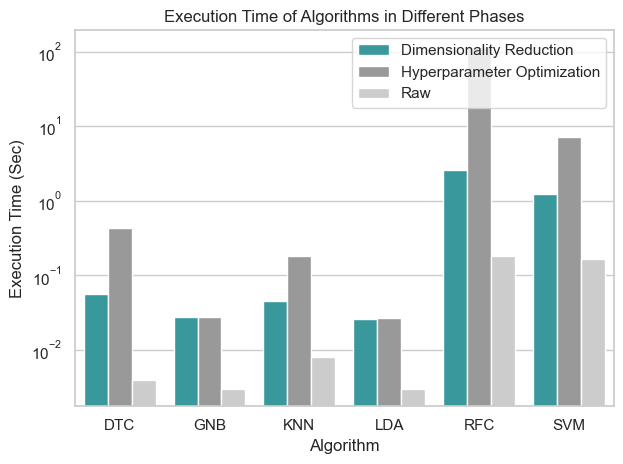
\includegraphics[width=\linewidth]{Plots/ExecutionTimeofAlgorithmsinDifferentPhases.png}
        \caption{Execution time}
        \label{fig:executionTimeOfAlgorithmsInDifferentphases}
    \end{subfigure}
    
    \caption{Algorithm performance in different phases}
\end{figure}

%%%%%%%%%%%%%% Discussion %%%%%%%%%%%%%%
\section{Discussion}













\newpage
\appendix

% \begin{figure}[H]
%     \centering   
%     \begin{subfigure}{0.4\textwidth}
% 		\centering
% 		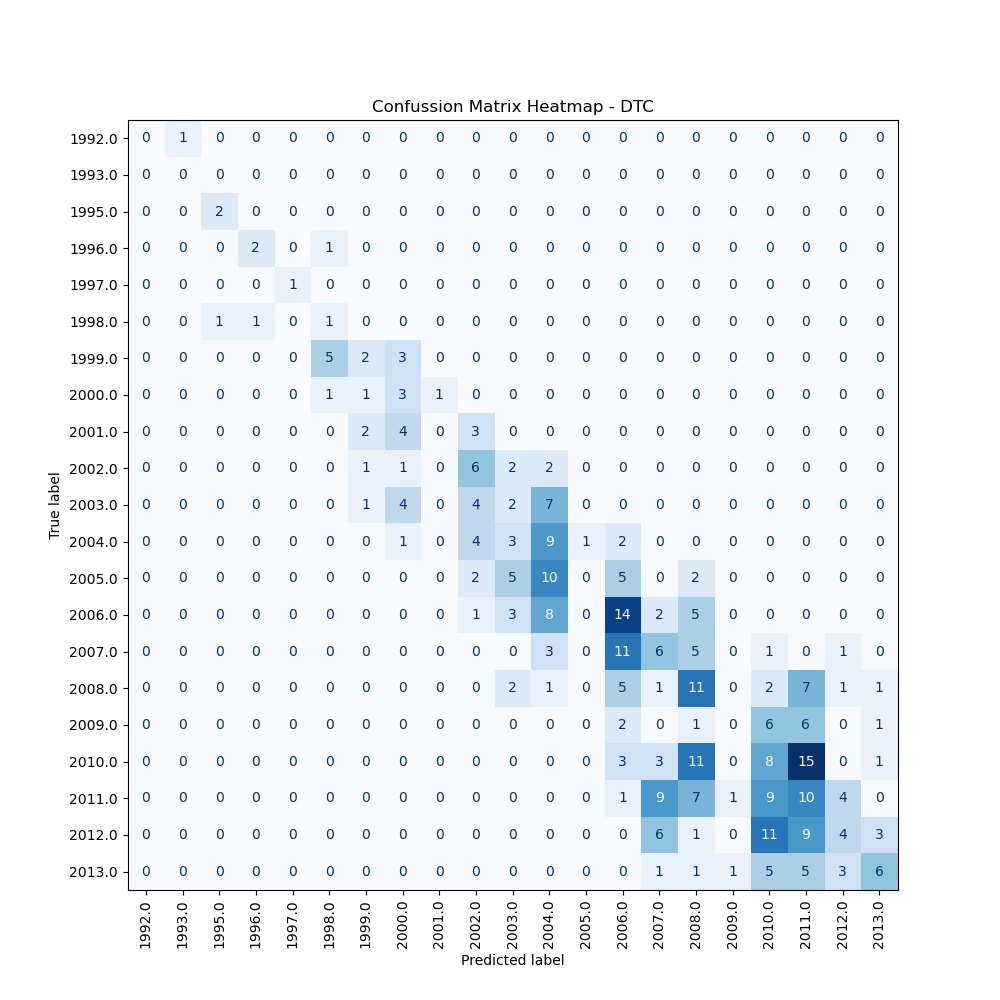
\includegraphics[width=\linewidth]{Plots/CM_Heatmap_DTC.png}
% 		\caption{Confusion matrix of the DTC (optimized))}
% 		\label{appdx:cmheatmapdtc}
% 	\end{subfigure}

% 	\begin{subfigure}{0.4\textwidth}
% 		\centering
% 		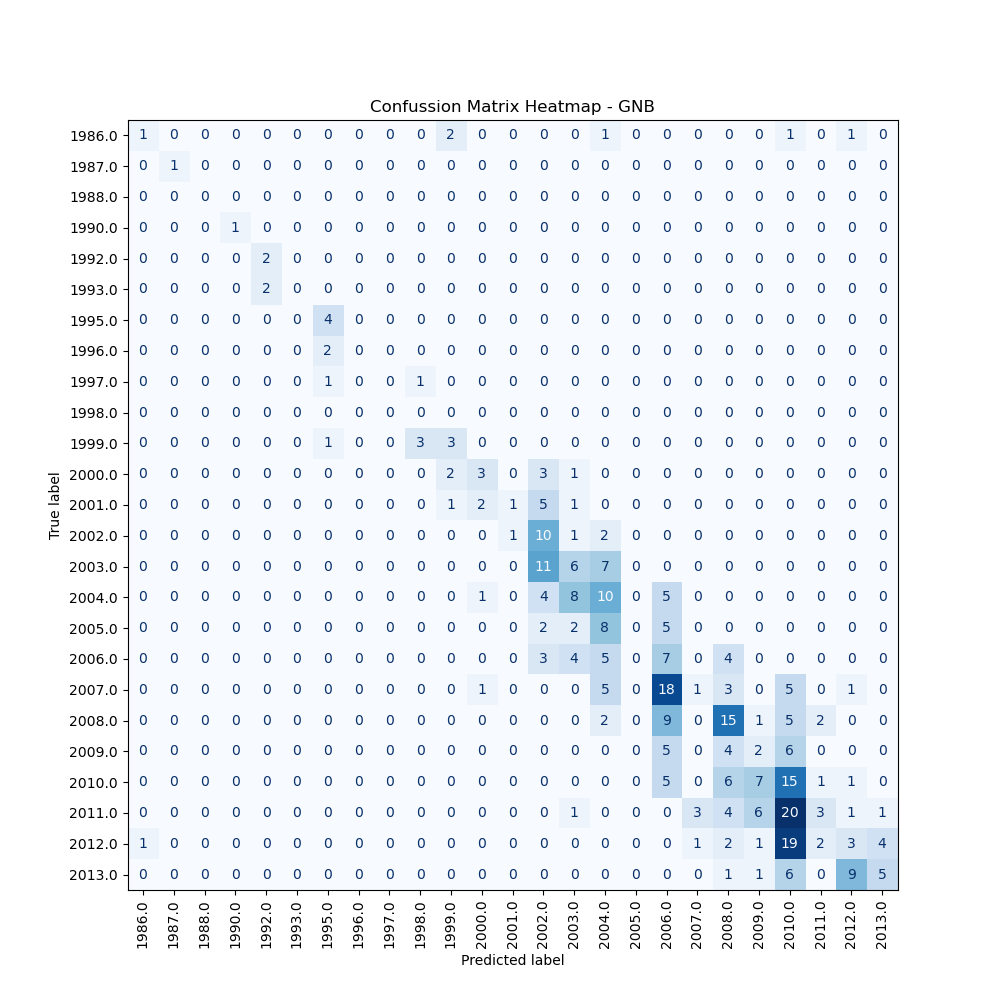
\includegraphics[width=\linewidth]{Plots/CM_Heatmap_GNB.png}
% 		\caption{Confusion matrix of the GNB (optimized))}
% 		\label{appx:cmheatmapgnb}
% 	\end{subfigure}

%     \begin{subfigure}{0.5\textwidth}
% 		\centering
% 		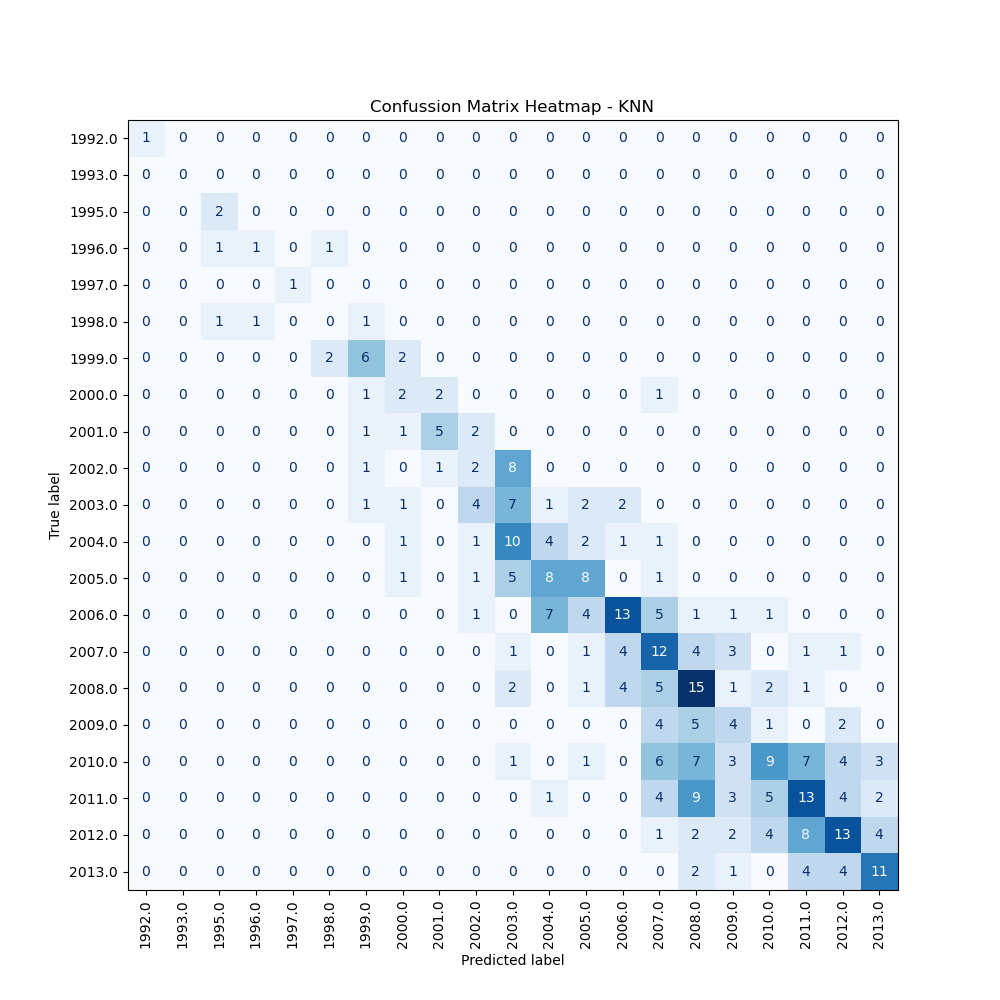
\includegraphics[width=\linewidth]{Plots/CM_Heatmap_KNN.png}
% 		\caption{Confusion matrix of the KNN (optimized))}
% 		\label{appx:cmheatmapknn}
% 	\end{subfigure}

%     \begin{subfigure}{0.5\textwidth}
% 		\centering
% 		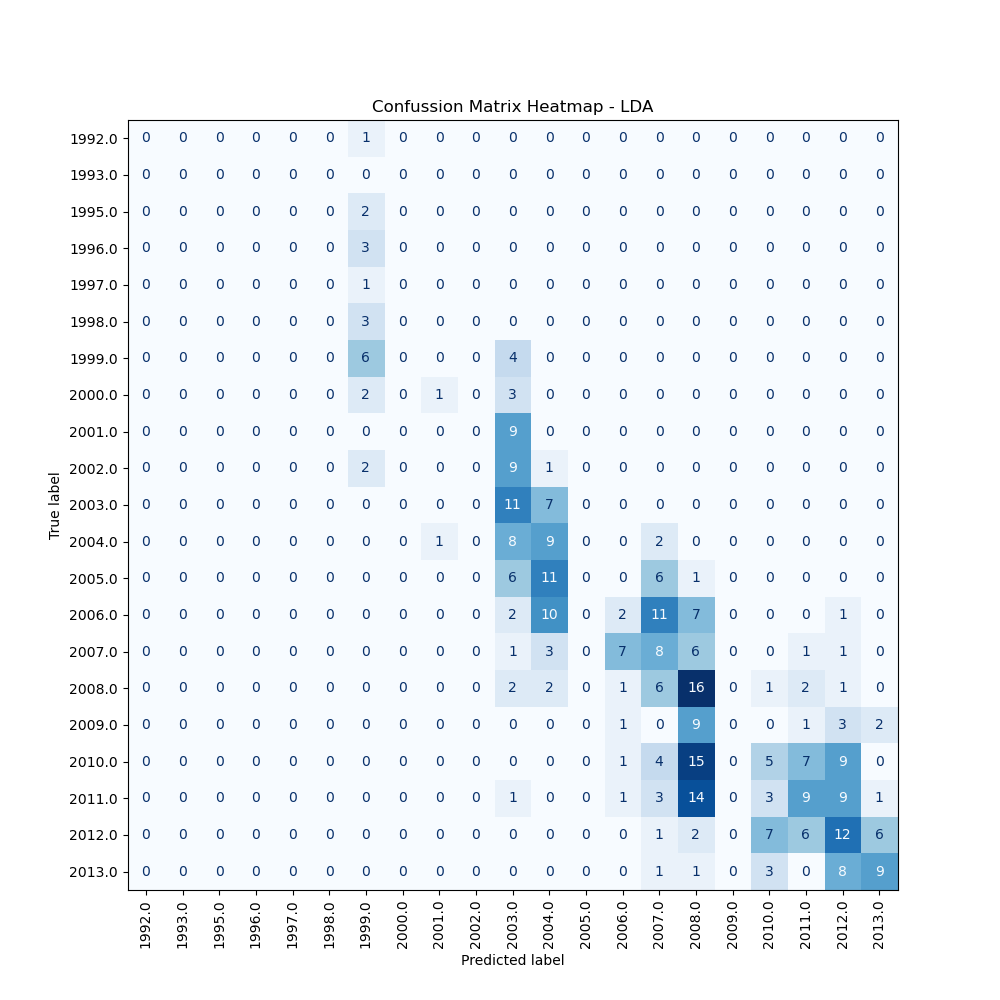
\includegraphics[width=\linewidth]{Plots/CM_Heatmap_LDA.png}
% 		\caption{Confusion matrix of the LDA)}
% 		\label{appx:cmheatmaplda}
% 	\end{subfigure}

%     \begin{subfigure}{0.5\textwidth}
% 		\centering
% 		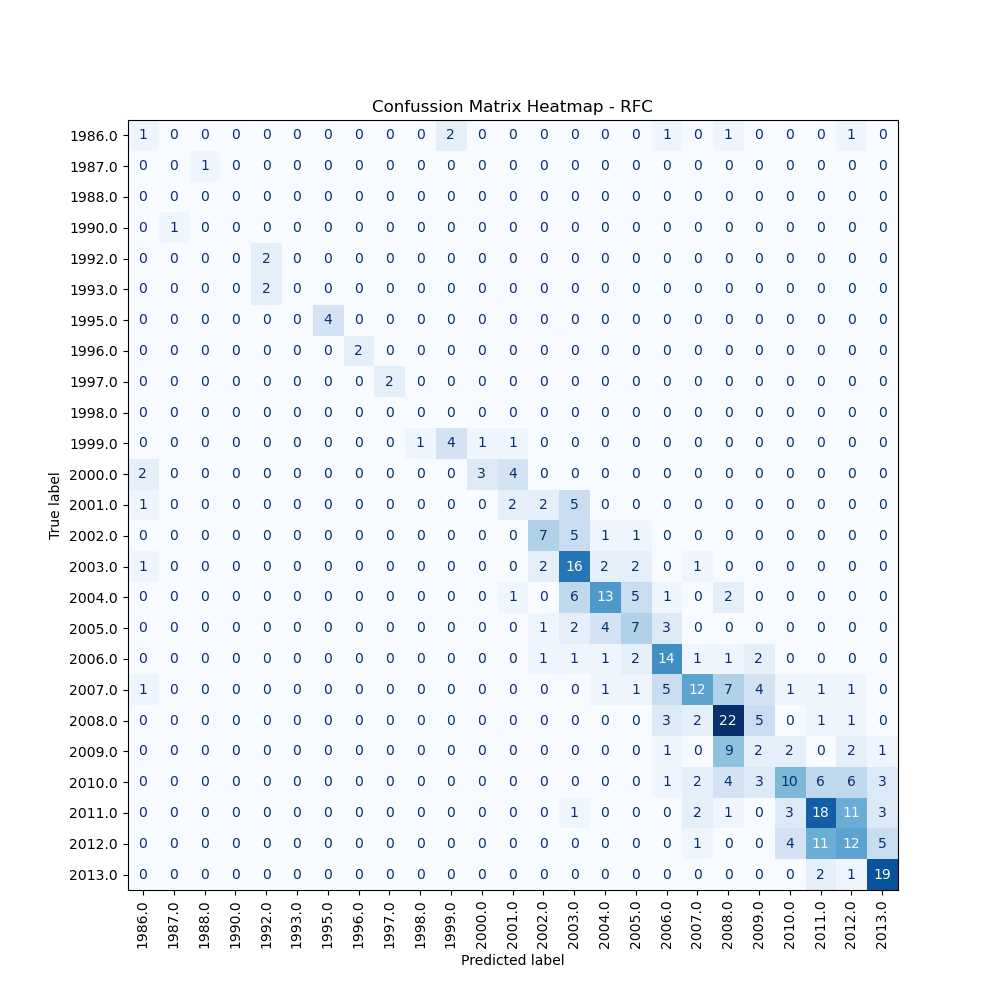
\includegraphics[width=\linewidth]{Plots/CM_Heatmap_RFC.png}
% 		\caption{Confusion matrix of the RFC (optimized))}
% 		\label{appx:cmheatmaprfc}
% 	\end{subfigure}

%     \begin{subfigure}{0.5\textwidth}
% 		\centering
% 		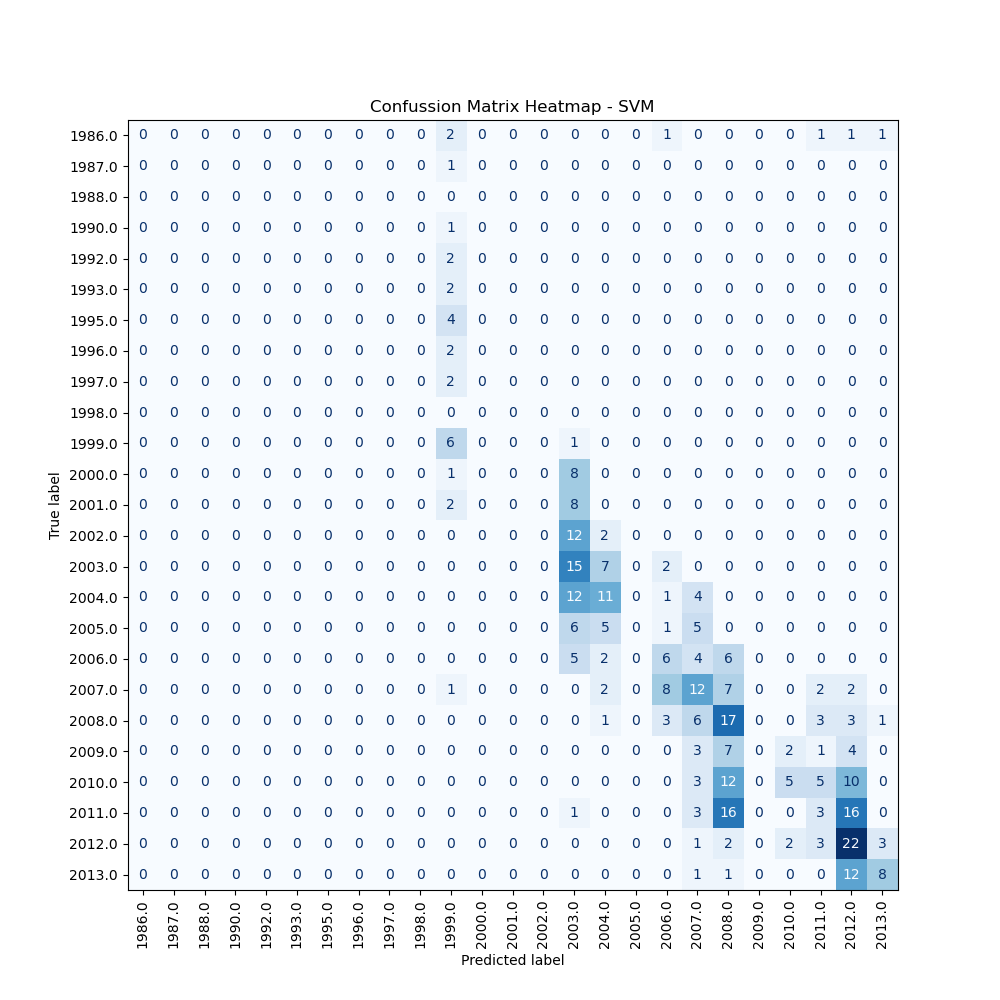
\includegraphics[width=\linewidth]{Plots/CM_Heatmap_SVM.png}
% 		\caption{Confusion matrix of the SVM (optimized))}
% 		\label{appx:cmheatmapsvm}
% 	\end{subfigure}

%     \caption{Algorithm performance in different phases}
% \end{figure}


\begin{figure}[htbp]
    \centering
    \begin{subfigure}{0.4\textwidth}
        \centering
		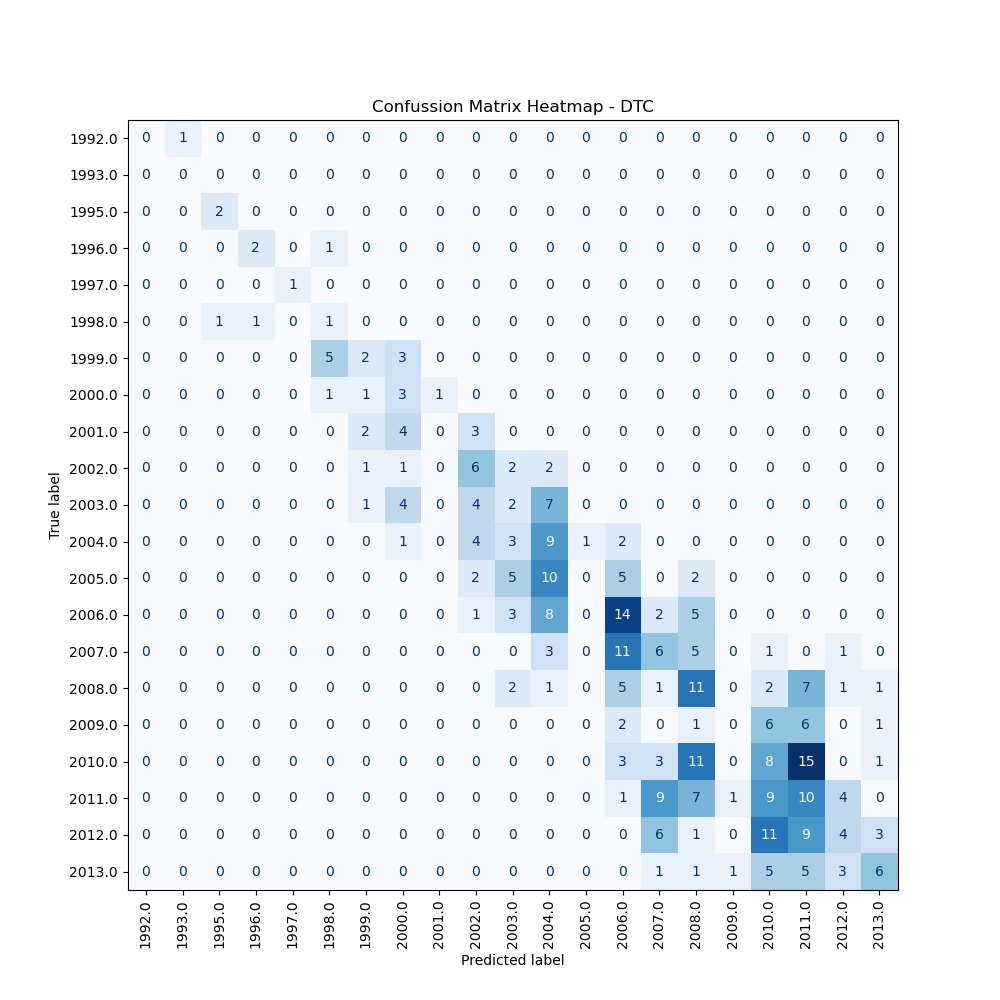
\includegraphics[width=\linewidth]{Plots/CM_Heatmap_DTC.png}
		\caption{DTC (optimized)}
		\label{appdx:cmheatmapdtc}
    \end{subfigure}%
    \begin{subfigure}{0.4\textwidth}
        \centering
		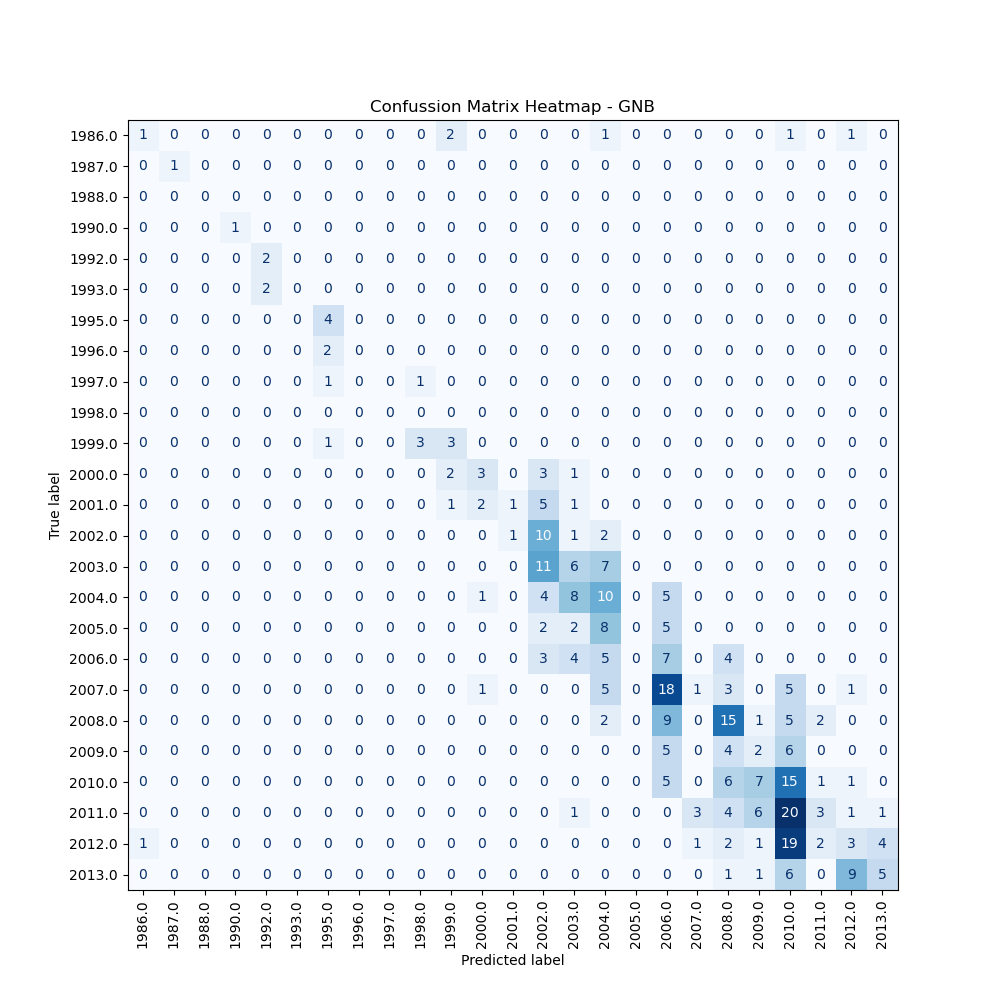
\includegraphics[width=\linewidth]{Plots/CM_Heatmap_GNB.png}
		\caption{GNB (optimized)}
		\label{appx:cmheatmapgnb}
    \end{subfigure}\\
    \begin{subfigure}{0.4\textwidth}
        \centering
		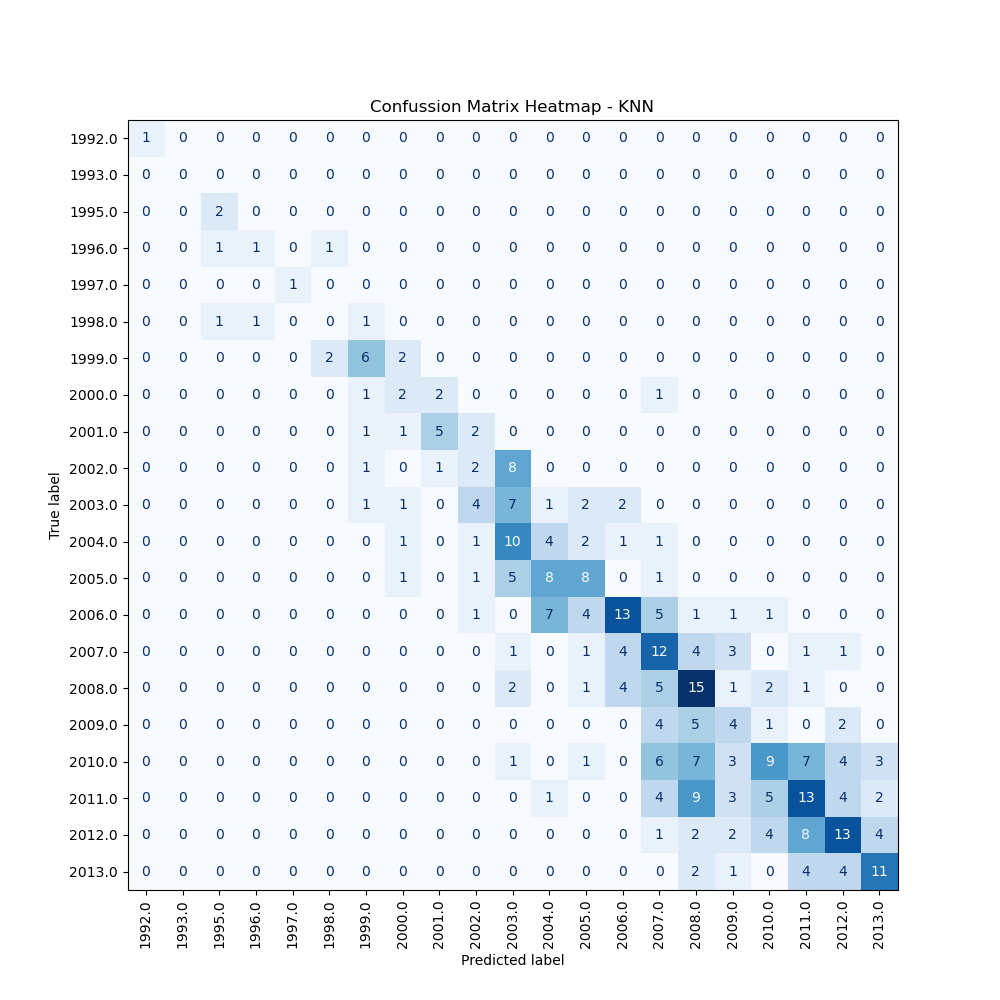
\includegraphics[width=\linewidth]{Plots/CM_Heatmap_KNN.png}
		\caption{KNN (optimized)}
		\label{appx:cmheatmapknn}
    \end{subfigure}%
    \begin{subfigure}{0.4\textwidth}
        \centering
		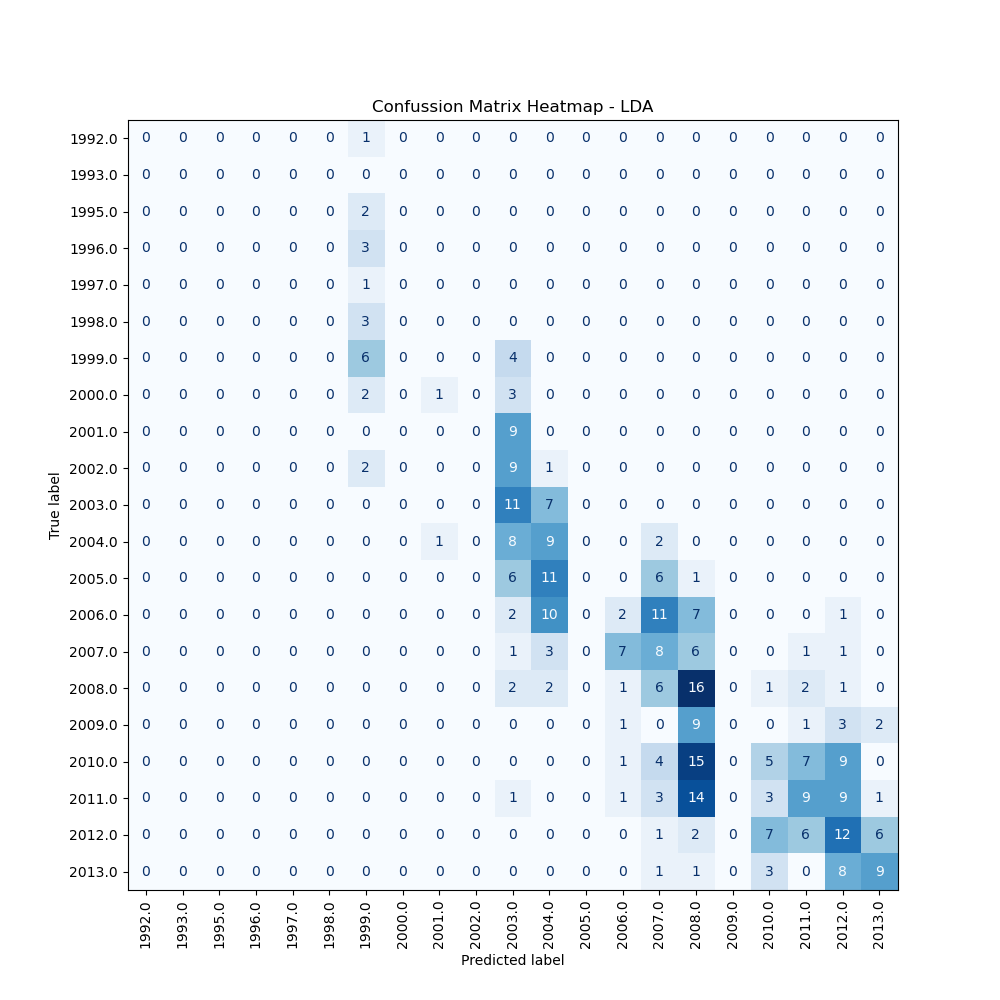
\includegraphics[width=\linewidth]{Plots/CM_Heatmap_LDA.png}
		\caption{LDA)}
		\label{appx:cmheatmaplda}
    \end{subfigure}\\
    \begin{subfigure}{0.4\textwidth}
        \centering
		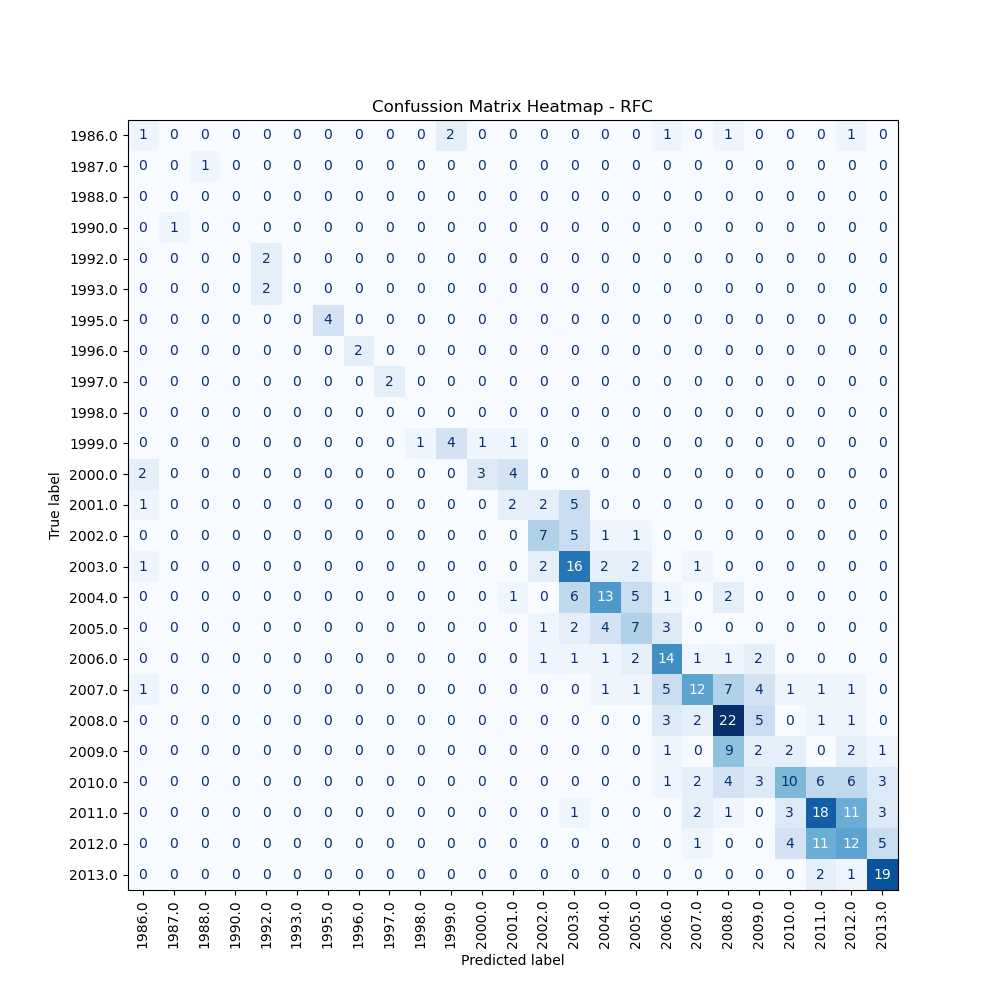
\includegraphics[width=\linewidth]{Plots/CM_Heatmap_RFC.png}
		\caption{RFC (optimized)}
		\label{appx:cmheatmaprfc}
    \end{subfigure}%
    \begin{subfigure}{0.4\textwidth}
        \centering
		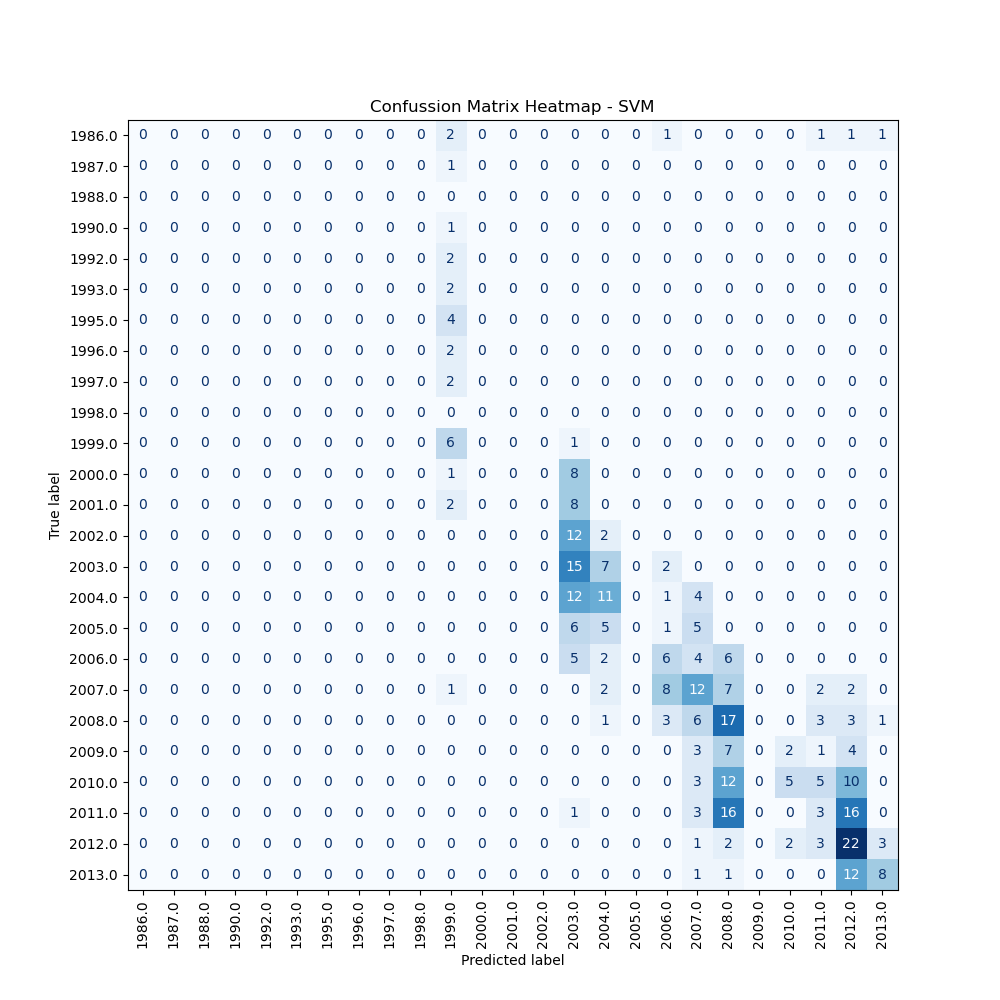
\includegraphics[width=\linewidth]{Plots/CM_Heatmap_SVM.png}
		\caption{SVM (optimized)}
		\label{appx:cmheatmapsvm}
    \end{subfigure}
    \caption{Confusion matrix of all the six classifiers}
    \label{appdx:confusionMatrixOfAllTheSixClassifiers}
\end{figure}

    \begin{longtable}{lrrrrrr}
        \hline
         Algorithm   &   CV\_Accuracy &   Accuracy &   Precision &   Recall &       F1 &   Execution Time \\ \hline
         RFC         &      0.440845 &   0.473239 &    0.482281 & 0.473239 & 0.467693 &       0.172644   \\
         DTC         &      0.400704 &   0.442254 &    0.449104 & 0.442254 & 0.435644 &       0.00341725 \\
         SVM         &      0.280986 &   0.28169  &    0.253084 & 0.28169  & 0.219221 &       0.157703   \\
         KNN         &      0.360563 &   0.357746 &    0.379279 & 0.357746 & 0.351769 &       0.00796819 \\
         LDA         &      0.261972 &   0.24507  &    0.205744 & 0.24507  & 0.202823 &       0.00258398 \\
         GNB         &      0.228873 &   0.205634 &    0.182054 & 0.205634 & 0.18264  &       0.00265884 \\
         RFC         &      0.440845 &   0.473239 &    0.482281 & 0.473239 & 0.467693 &       0.170908   \\
         DTC         &      0.400704 &   0.442254 &    0.449104 & 0.442254 & 0.435644 &       0.00406098 \\
         SVM         &      0.280986 &   0.28169  &    0.253084 & 0.28169  & 0.219221 &       0.161214   \\
         KNN         &      0.360563 &   0.357746 &    0.379279 & 0.357746 & 0.351769 &       0.0083189  \\
         LDA         &      0.261972 &   0.24507  &    0.205744 & 0.24507  & 0.202823 &       0.00339317 \\
         GNB         &      0.228873 &   0.205634 &    0.182054 & 0.205634 & 0.18264  &       0.00308394 \\
         RFC         &      0.440845 &   0.473239 &    0.482281 & 0.473239 & 0.467693 &       0.187191   \\
         DTC         &      0.400704 &   0.442254 &    0.449104 & 0.442254 & 0.435644 &       0.00370598 \\
         SVM         &      0.280986 &   0.28169  &    0.253084 & 0.28169  & 0.219221 &       0.16112    \\
         KNN         &      0.360563 &   0.357746 &    0.379279 & 0.357746 & 0.351769 &       0.00886011 \\
         LDA         &      0.261972 &   0.24507  &    0.205744 & 0.24507  & 0.202823 &       0.00250292 \\
         GNB         &      0.228873 &   0.205634 &    0.182054 & 0.205634 & 0.18264  &       0.00361419 \\
        \hline
        \caption{State-of-the-art classifiers performance}
        \label{appdx:stateOfTheArtClassifiersPerformance}
    \end{longtable}
        
    \begin{longtable}{lrrrrrr}
        \hline
         Algorithm   &   CV\_Accuracy &   Accuracy &   Precision &   Recall &       F1 &   Execution Time \\
        \hline
         RFC         &      0.407746 &   0.439437 &    0.45987  & 0.439437 & 0.437043 &        1.25214   \\
         DTC         &      0.371127 &   0.422535 &    0.435677 & 0.422535 & 0.422189 &        0.0277729 \\
         SVM         &      0.311972 &   0.309859 &    0.2939   & 0.309859 & 0.266544 &        0.665152  \\
         KNN         &      0.376761 &   0.36338  &    0.384735 & 0.36338  & 0.363729 &        0.0385151 \\
         LDA         &      0.261268 &   0.24507  &    0.205744 & 0.24507  & 0.202823 &        0.0127187 \\
         GNB         &      0.273239 &   0.24507  &    0.224912 & 0.24507  & 0.221897 &        0.0145471 \\
         RFC         &      0.407746 &   0.439437 &    0.45987  & 0.439437 & 0.437043 &        1.25332   \\
         DTC         &      0.371127 &   0.422535 &    0.435677 & 0.422535 & 0.422189 &        0.0303597 \\
         SVM         &      0.311972 &   0.309859 &    0.2939   & 0.309859 & 0.266544 &        0.67257   \\
         KNN         &      0.376761 &   0.36338  &    0.384735 & 0.36338  & 0.363729 &        0.0449691 \\
         LDA         &      0.261268 &   0.24507  &    0.205744 & 0.24507  & 0.202823 &        0.0141079 \\
         GNB         &      0.273239 &   0.24507  &    0.224912 & 0.24507  & 0.221897 &        0.01702   \\
         RFC         &      0.407746 &   0.439437 &    0.45987  & 0.439437 & 0.437043 &        1.36698   \\
         DTC         &      0.371127 &   0.422535 &    0.435677 & 0.422535 & 0.422189 &        0.0315924 \\
         SVM         &      0.311972 &   0.309859 &    0.2939   & 0.309859 & 0.266544 &        0.686508  \\
         KNN         &      0.376761 &   0.36338  &    0.384735 & 0.36338  & 0.363729 &        0.0410869 \\
         LDA         &      0.261268 &   0.24507  &    0.205744 & 0.24507  & 0.202823 &        0.013967  \\
         GNB         &      0.273239 &   0.24507  &    0.224912 & 0.24507  & 0.221897 &        0.0185232 \\
        \hline
        \caption{Classifiers performance after dimensionality reduction}
        \label{appdx:classifierPerformanceAfterDimensionalityReduction}
    \end{longtable}
            
    \begin{longtable}{lrrrrrr}
        \hline
         Algorithm   &   CV\_Accuracy &   Accuracy &   Precision &   Recall &       F1 &   Execution Time \\
        \hline
         RFC         &      0.423239 &   0.459155 &    0.487308 & 0.459155 & 0.456431 &       51.2526    \\
         DTC         &      0.378873 &   0.430986 &    0.444931 & 0.430986 & 0.428687 &        0.193149  \\
         SVM         &      0.361972 &   0.394366 &    0.368064 & 0.394366 & 0.363465 &        3.54028   \\
         KNN         &      0.417606 &   0.450704 &    0.465625 & 0.450704 & 0.445552 &        0.133158  \\
         LDA         &      0.261268 &   0.24507  &    0.205744 & 0.24507  & 0.202823 &        0.0122411 \\
         GNB         &      0.273239 &   0.24507  &    0.224912 & 0.24507  & 0.221897 &        0.015172  \\
         RFC         &      0.423239 &   0.459155 &    0.487308 & 0.459155 & 0.456431 &       52.1694    \\
         DTC         &      0.378873 &   0.430986 &    0.444931 & 0.430986 & 0.428687 &        0.204587  \\
         SVM         &      0.361972 &   0.394366 &    0.368064 & 0.394366 & 0.363465 &        3.50349   \\
         KNN         &      0.417606 &   0.450704 &    0.465625 & 0.450704 & 0.445552 &        0.154317  \\
         LDA         &      0.261268 &   0.24507  &    0.205744 & 0.24507  & 0.202823 &        0.0139561 \\
         GNB         &      0.273239 &   0.24507  &    0.224912 & 0.24507  & 0.221897 &        0.018435  \\
         RFC         &      0.423239 &   0.459155 &    0.487308 & 0.459155 & 0.456431 &       56.1888    \\
         DTC         &      0.378873 &   0.430986 &    0.444931 & 0.430986 & 0.428687 &        0.209001  \\
         SVM         &      0.361972 &   0.394366 &    0.368064 & 0.394366 & 0.363465 &        3.53441   \\
         KNN         &      0.417606 &   0.450704 &    0.465625 & 0.450704 & 0.445552 &        0.142963  \\
         LDA         &      0.261268 &   0.24507  &    0.205744 & 0.24507  & 0.202823 &        0.0146387 \\
         GNB         &      0.273239 &   0.24507  &    0.224912 & 0.24507  & 0.221897 &        0.0194271 \\
        \hline
        \caption{Classifiers performance after dimensionality reduction and hyperparameter optimization}
        \label{appdx:classifierPerformanceAfterDimensionalityReductionAndHyperparameterOptimization}
    \end{longtable}


    \begin{table}[H]
        \begin{center}
        \begin{longtable}{lrrl}
            \hline
             Classifier   &   Accuracy &   Std test score & params                                                            \\
            \hline
             RFC          &   0.407746 &       0.0120749  & \{'max\_depth': None, 'min\_samples\_split': 2, 'n\_estimators': 100\}  \\
             RFC          &   0.412676 &       0.0128702  & \{'max\_depth': None, 'min\_samples\_split': 2, 'n\_estimators': 200\}  \\
             RFC          &   0.414789 &       0.0124789  & \{'max\_depth': None, 'min\_samples\_split': 2, 'n\_estimators': 300\}  \\
             RFC          &   0.415493 &       0.0231432  & \{'max\_depth': None, 'min\_samples\_split': 5, 'n\_estimators': 100\}  \\
             RFC          &   0.416197 &       0.0257211  & \{'max\_depth': None, 'min\_samples\_split': 5, 'n\_estimators': 200\}  \\
             RFC          &   0.419014 &       0.0202885  & \{'max\_depth': None, 'min\_samples\_split': 5, 'n\_estimators': 300\}  \\
             RFC          &   0.405634 &       0.0219782  & \{'max\_depth': None, 'min\_samples\_split': 10, 'n\_estimators': 100\} \\
             RFC          &   0.409859 &       0.0155249  & \{'max\_depth': None, 'min\_samples\_split': 10, 'n\_estimators': 200\} \\
             RFC          &   0.409155 &       0.0211737  & \{'max\_depth': None, 'min\_samples\_split': 10, 'n\_estimators': 300\} \\
             RFC          &   0.419014 &       0.0131748  & \{'max\_depth': 10, 'min\_samples\_split': 2, 'n\_estimators': 100\}    \\
             RFC          &   0.423239 &       0.00928937 & \{'max\_depth': 10, 'min\_samples\_split': 2, 'n\_estimators': 200\}    \\
             RFC          &   0.423239 &       0.0112235  & \{'max\_depth': 10, 'min\_samples\_split': 2, 'n\_estimators': 300\}    \\
             RFC          &   0.414085 &       0.0125186  & \{'max\_depth': 10, 'min\_samples\_split': 5, 'n\_estimators': 100\}    \\
             RFC          &   0.416901 &       0.0138358  & \{'max\_depth': 10, 'min\_samples\_split': 5, 'n\_estimators': 200\}    \\
             RFC          &   0.419718 &       0.0164252  & \{'max\_depth': 10, 'min\_samples\_split': 5, 'n\_estimators': 300\}    \\
             RFC          &   0.4      &       0.0181739  & \{'max\_depth': 10, 'min\_samples\_split': 10, 'n\_estimators': 100\}   \\
             RFC          &   0.400704 &       0.0193374  & \{'max\_depth': 10, 'min\_samples\_split': 10, 'n\_estimators': 200\}   \\
             RFC          &   0.405634 &       0.0210562  & \{'max\_depth': 10, 'min\_samples\_split': 10, 'n\_estimators': 300\}   \\
             RFC          &   0.407746 &       0.0145009  & \{'max\_depth': 20, 'min\_samples\_split': 2, 'n\_estimators': 100\}    \\
             RFC          &   0.414789 &       0.0177319  & \{'max\_depth': 20, 'min\_samples\_split': 2, 'n\_estimators': 200\}    \\
             RFC          &   0.416901 &       0.0167541  & \{'max\_depth': 20, 'min\_samples\_split': 2, 'n\_estimators': 300\}    \\
             RFC          &   0.414085 &       0.024456   & \{'max\_depth': 20, 'min\_samples\_split': 5, 'n\_estimators': 100\}    \\
             RFC          &   0.414789 &       0.0235047  & \{'max\_depth': 20, 'min\_samples\_split': 5, 'n\_estimators': 200\}    \\
             RFC          &   0.417606 &       0.0208432  & \{'max\_depth': 20, 'min\_samples\_split': 5, 'n\_estimators': 300\}    \\
             RFC          &   0.406338 &       0.0232074  & \{'max\_depth': 20, 'min\_samples\_split': 10, 'n\_estimators': 100\}   \\
             RFC          &   0.407746 &       0.0151695  & \{'max\_depth': 20, 'min\_samples\_split': 10, 'n\_estimators': 200\}   \\
             RFC          &   0.408451 &       0.0200426  & \{'max\_depth': 20, 'min\_samples\_split': 10, 'n\_estimators': 300\}   \\
             DTC          &   0.371127 &       0.0119095  & \{'max\_depth': None, 'min\_samples\_split': 2\}                       \\
             DTC          &   0.378169 &       0.0187117  & \{'max\_depth': None, 'min\_samples\_split': 5\}                       \\
             DTC          &   0.357042 &       0.0208432  & \{'max\_depth': None, 'min\_samples\_split': 10\}                      \\
             DTC          &   0.359155 &       0.0248981  & \{'max\_depth': 10, 'min\_samples\_split': 2\}                         \\
             DTC          &   0.358451 &       0.0241294  & \{'max\_depth': 10, 'min\_samples\_split': 5\}                         \\
             DTC          &   0.347887 &       0.0175915  & \{'max\_depth': 10, 'min\_samples\_split': 10\}                        \\
             DTC          &   0.376056 &       0.0167244  & \{'max\_depth': 20, 'min\_samples\_split': 2\}                         \\
             DTC          &   0.378873 &       0.0214298  & \{'max\_depth': 20, 'min\_samples\_split': 5\}                         \\
             DTC          &   0.357042 &       0.0208432  & \{'max\_depth': 20, 'min\_samples\_split': 10\}                        \\
             SVM          &   0.259155 &       0.00653072 & \{'C': 0.1, 'gamma': 'scale'\}                                      \\
             SVM          &   0.257042 &       0.00995925 & \{'C': 0.1, 'gamma': 'auto'\}                                       \\
             SVM          &   0.311972 &       0.0192345  & \{'C': 1, 'gamma': 'scale'\}                                        \\
             SVM          &   0.316197 &       0.0189488  & \{'C': 1, 'gamma': 'auto'\}                                         \\
             SVM          &   0.360563 &       0.0176197  & \{'C': 10, 'gamma': 'scale'\}                                       \\
             SVM          &   0.361972 &       0.0165755  & \{'C': 10, 'gamma': 'auto'\}                                        \\
             KNN          &   0.390141 &       0.0205798  & \{'n\_neighbors': 3, 'weights': 'uniform'\}                          \\
             KNN          &   0.407042 &       0.0203617  & \{'n\_neighbors': 3, 'weights': 'distance'\}                         \\
             KNN          &   0.376761 &       0.0175351  & \{'n\_neighbors': 5, 'weights': 'uniform'\}                          \\
             KNN          &   0.411972 &       0.0125976  & \{'n\_neighbors': 5, 'weights': 'distance'\}                         \\
             KNN          &   0.373239 &       0.0159036  & \{'n\_neighbors': 7, 'weights': 'uniform'\}                          \\
             KNN          &   0.417606 &       0.0176197  & \{'n\_neighbors': 7, 'weights': 'distance'\}                         \\
             LDA          &   0.261268 &       0.0222027  & \{\}                                                                \\
             GNB          &   0.273239 &       0.0181739  & \{\}                                                                \\
            \hline
        \end{longtable}
        \caption{Possible combination of the best parameters for each classifier}
        \label{appdx:bestParameters}
        \end{center}
    \end{table}
        
\begin{figure}[H]
    \centering
    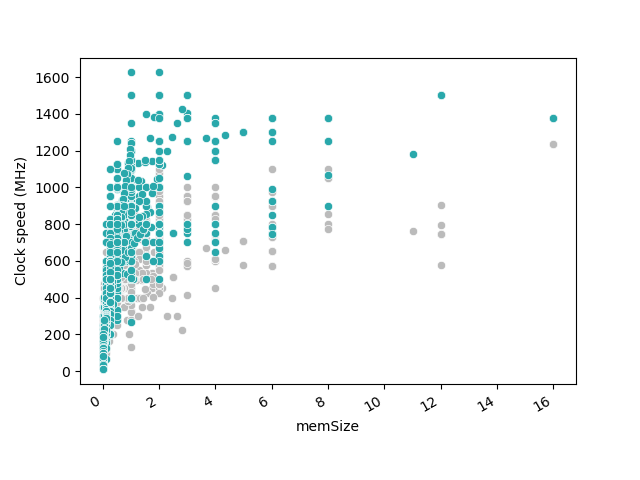
\includegraphics[width=0.7\textwidth]{Plots/DatagpuClockvsmemClock.png}
    \caption{GPU release year vs GPU memory clock}
    \label{appdx:gpuReleaseYearvsGPUMemoryClock}
\end{figure}

\begin{figure}[H]
    \centering
    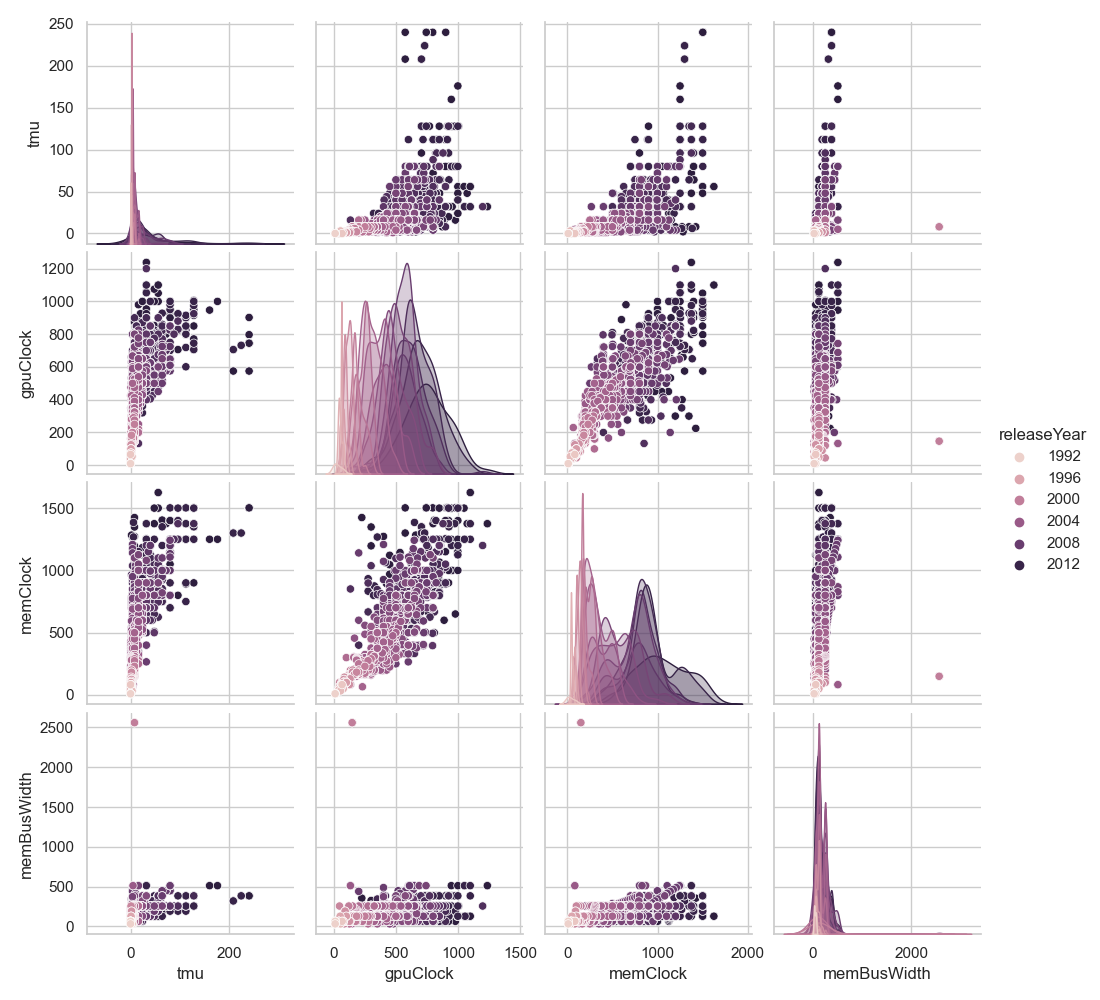
\includegraphics[width=0.7\textwidth]{Plots/DataPariPlot.png}
    \caption{Parallel plot of the data}
    \label{appdx:parallelPlotOfTheData}
\end{figure}

\newpage
\bibliographystyle{IEEEtran}
\bibliography{ref}
\end{document}